\begin{figure*}[t]
\centering
\resizebox{\linewidth}{!}{%
\begin{tikzpicture}[
  font=\scriptsize, >=stealth, node distance=4mm,
  box/.style={draw, rounded corners=2pt, align=center, minimum height=7mm, inner sep=2pt, fill=white},
  data/.style={box, fill=gray!10},
  net/.style={box, fill=blue!8},
  sim/.style={box, fill=orange!12},
  loop/.style={draw, dashed, rounded corners=4pt, inner sep=3pt, blue!50!black}]
% inputs, each tokenised in its canonical frame and encoded with local attention
\node[data, text width=24mm] (A) {snapshot $a$:\\$\{\mathbf{x}_i\}_{i\le N_a}$, tokens + local attention};
\node[data, text width=24mm, below=5mm of A] (B) {snapshot $b{=}a{+}H$:\\$\{\mathbf{y}_j\}_{j\le N_b}$, tokens + local attention};
\node[data, text width=24mm, below=4mm of B] (I) {image at $b$};
% loop: X1 -> U -> X2 -> X1
\node[net, right=15mm of A] (X1) {(i, ii) ancestors attend\\to targets near $\mathbf{c}_i^{(t-1)}$};
\node[net, right=4mm of X1] (U) {(iii) $\mathbf{c}_i^{(t)}{=}\mathbf{c}_i^{(t-1)}{+}\Delta_t$};
\node[net, below=5mm of X1] (X2) {(iv) targets attend\\to nearest centres};
\node[loop, fit=(X1)(U)(X2), label={[blue!50!black, font=\scriptsize]below right:{family registration, $t{=}1..T$}}] (L) {};
\node[net, right=6mm of U] (S) {scores $p_{ji}$\\+ dustbin};
\node[net, right=4mm of S] (P) {Potts mean\\field (Eq.~1)};
\node[box, right=4mm of P] (O) {ancestor\\$\pi(j)$};
% genealogy
\node[net, right=6mm of I] (G) {pair CNN: $P(\tau_{jk}{<}H)$};
% real-data inset: centres moving through the rounds
\node[anchor=north west, inner sep=0] (IN) at ([xshift=4mm, yshift=-3mm]O.north east) {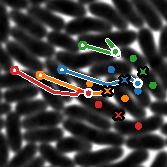
\includegraphics[height=29mm]{fig/centre_inset.pdf}};
\node[anchor=south, font=\scriptsize] at (IN.north) {real data, $H{=}66$ min};
\draw[->] (A) -- node[above, font=\scriptsize] {$\mathbf{c}^{(0)}_i$} node[below, font=\tiny] {radial/Darcy} (X1);
\draw[->] (I) -- (G);
\draw[->] (X1) -- (U);
\draw[->] (U.south) |- (X2.east); \draw[->] (X2.north) -- (X1.south);
\draw[->] (B) -- (X2);
\draw[->] (U) -- (S); \draw[->] (S) -- (P); \draw[->] (G) -| (P); \draw[->] (P) -- (O);
\end{tikzpicture}}
\caption{\textbf{Overview.} For every ancestor \ours keeps one estimate of its descendant-family centre and refines it over $T$ rounds of cross-attention to nearby targets; targets then score candidate ancestors by their offset from the refined centres. A genealogy network predicts from the target image whether neighbouring cells share an ancestor $H$ minutes ago, and a Potts mean-field decoder combines both. The same network is trained on \rodsim colonies, self-labelled time-lapses or annotated lineage. Right: in a dense OIAM window, centres move from initialisation (open) to $\mathbf{c}_i^{(T)}$ (filled) towards the true centroids (crosses) of the descendants (dots).}
\label{fig:method}
\end{figure*}
